\chapter{Expérience 1 : Séance de rétro-ingénierie pour l'apprentissage du SQL}

\section{Axe 1 : Contexte et intentions pédagogiques}

\subsection{Public et niveau}

Cette séance s'adresse à des élèves de \textbf{Terminale NSI} (Numérique et Sciences Informatiques) \parencite{baccalaureat_nsi}, possédant les notions de base sur le modèle relationnel vues en classe de Première. L'effectif est d'environ 25 élèves, avec des niveaux hétérogènes en programmation mais une certaine familiarité avec les concepts de base de données.

Le programme officiel de NSI \parencite{eduscol_nsi,nsi_programmes} prévoit en terminale l'approfondissement des bases de données relationnelles, incluant la maîtrise du langage SQL pour la création, la manipulation et l'interrogation de bases de données.

\subsection{Objectifs d'apprentissage}

Les objectifs, reformulés selon la \textbf{Taxonomie de Bloom} \parencite{bloom_taxonomy,anderson_bloom_revised}, visent à mobiliser des niveaux cognitifs élevés, dépassant la simple application technique :

\begin{itemize}[leftmargin=*]
    \item \textbf{Niveau 1 - Connaissance} : Identifier les commandes SQL fondamentales (SELECT, WHERE, JOIN) et le vocabulaire spécifique (table, attribut, clé primaire).
    \item \textbf{Niveau 2 - Compréhension} : Expliquer la nécessité de la normalisation pour éviter la redondance et garantir la cohérence des données.
    \item \textbf{Niveau 3 - Application} : Écrire des requêtes simples pour extraire des informations ciblées d'une base existante.
    \item \textbf{Niveau 4 - Analyse} : Déduire le schéma relationnel (tables et relations) à partir de l'observation des données brutes et de l'interface du site web (démarche de rétro-ingénierie).
    \item \textbf{Niveau 5 - Synthèse} : Reconstruire le modèle conceptuel global du système d'information à partir des fragments analysés.
    \item \textbf{Niveau 6 - Évaluation} : Juger de la pertinence d'un choix de modélisation (ex: choix de la clé primaire) ou de la structure proposée par un pair.
\end{itemize}

Cette structuration montre que la rétro-ingénierie sollicite particulièrement les niveaux supérieurs d'analyse et de synthèse, favorisant une compréhension profonde des concepts.

\subsection{Support pédagogique et choix didactique}

Le choix stratégique d'utiliser mon site personnel \texttt{pytel.fr/site/} garantit un \textbf{environnement d'apprentissage stable et maîtrisé}. Ce site contient des données structurées que j'ai préparées en amont, incluant volontairement les requêtes SQL directement visibles dans le code source, comme éléments à découvrir par les élèves.

\begin{figure}[H]
    \centering
    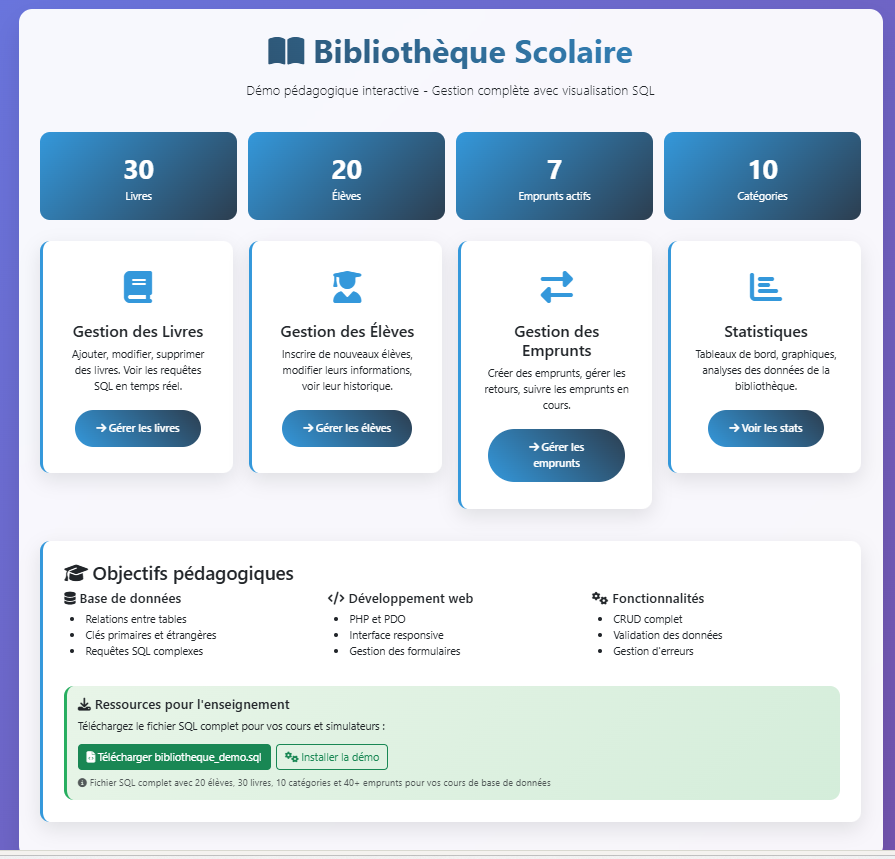
\includegraphics[width=0.9\textwidth]{annexes/pedagogiques/productions/site-sql.png}
    \caption{Capture d'écran de l'application "Bibliothèque Scolaire" utilisée pour la séance de rétro-ingénierie.}
    \label{fig-site-sql}
\end{figure}

Cette approche par \textbf{rétro-ingénierie} (illustrée par la Figure \ref{fig-site-sql}) constitue une transposition didactique originale \parencite{chevallard_transposition}. Plutôt que de partir du concept abstrait (le modèle relationnel) vers l'implémentation (le code SQL), je propose l'inverse : partir d'un système concret et fonctionnel pour en déduire les principes de conception.

Cette inversion pédagogique trouve ses fondements théoriques dans l'apprentissage par investigation \parencite{investigation_mathia,investigation_edutechwiki}, qui favorise l'engagement cognitif actif des élèves. Le processus d'apprentissage suit ainsi le cycle d'expérience de Kolb et les principes constructivistes de Vygotsky \parencite{vygotsky_mind_society,constructivisme_education,dale_cone}.

\section{Axe 2 : Déroulement concret de la séquence (2 heures)}

\subsection{Phase 1 - Exploration libre du système (20 minutes en binômes)}

Les élèves explorent le site avec pour consigne de « lister et décrire les informations présentes comme si vous deviez l'expliquer à un novice ». Cette phase de découverte génère des productions variées :

\begin{itemize}[leftmargin=*]
    \item Schémas conceptuels dessinés à la main
    \item Diagrammes de flux d'informations
    \item Descriptions textuelles structurées
    \item Ébauches de structures de tables (pour les plus avancés)
\end{itemize}

Cette diversité des productions révèle déjà les différentes stratégies cognitives des élèves face à un problème ouvert. Le travail en binômes hétérogènes favorise la verbalisation des raisonnements et la confrontation des idées, conformément aux principes de l'apprentissage collaboratif \parencite{apprentissage_collaboratif,vygotsky_mind_society}.

\subsection{Phase 2 - Abstraction et modélisation collective (40 minutes)}

J'anime une discussion collective en posant la question centrale : \textit{« Comment, en tant que concepteur, auriez-vous organisé ces informations ? »}

Cette interrogation amène naturellement les élèves à réfléchir aux problématiques de :
\begin{itemize}[leftmargin=*]
    \item \textbf{Redondance} : « Pourquoi ne pas répéter le nom de l'auteur dans chaque article ? »
    \item \textbf{Intégrité} : « Que se passe-t-il si on modifie le nom d'un auteur à un seul endroit ? »
    \item \textbf{Organisation} : « Quelles informations regrouper ensemble ? Selon quels critères ? »
\end{itemize}

J'introduis alors la notion de \textbf{clé primaire} par une analogie parlante. Du point de vue du \textbf{multi-agenda de Bucheton} \parencite{bucheton_postures}, cette phase constitue un moment critique de \textbf{tissage}. Mon activité d'enseignant vise ici à relier l'expérience immédiate et sensible des élèves (le désordre apparent des données, les doublons) aux savoirs savants abstraits (la théorie relationnelle et l'unicité de la clé).

Je maintiens simultanément une préoccupation de \textbf{pilotage} serré pour avancer dans la séance, tout en soignant l'\textbf{atmosphère} pour que les élèves osent formuler des hypothèses, même erronées. L'analogie sert ici d'instrument de tissage pour donner du sens aux concepts techniques.

\subsection{Phase 3 - Découverte guidée du SQL (60 minutes)}

Les élèves découvrent les requêtes SQL directement intégrées dans le code source du site. Dans un premier temps, ils doivent en déduire le fonctionnement « à l'instinct », ce qui favorise une \textbf{approche intuitive} du langage avant sa formalisation.

Cette phase génère beaucoup d'échanges spontanés et d'hypothèses. Je formalise ensuite l'apprentissage en :
\begin{enumerate}[leftmargin=*]
    \item Distribuant un glossaire des instructions SQL essentielles
    \item Explicitant la syntaxe générale (SELECT...FROM...WHERE...)
    \item Présentant le fichier de création des tables, permettant de comprendre la cohérence entre structure et requêtes
\end{enumerate}

Cette progression du concret vers l'abstrait respecte le cycle d'apprentissage de Kolb et le principe de construction progressive des savoirs \parencite{dale_cone,constructivisme_education}.

\section{Axe 3 : Résultats et évaluation formative}

\subsection{Productions initiales hétéroclites}

Les premiers schémas papier sont très divers, ce qui me permet de \textbf{diagnostiquer en temps réel} les niveaux de compréhension et les représentations mentales des élèves \parencite{evaluation_formative} :

\begin{itemize}[leftmargin=*]
    \item \textbf{Représentation linéaire} : Certains élèves proposent une seule grande table avec toutes les informations (erreur classique de redondance)
    \item \textbf{Représentation partielle} : D'autres identifient spontanément plusieurs entités mais sans les liens entre elles
    \item \textbf{Représentation avancée} : Quelques élèves proposent déjà des structures relationnelles avec identification des relations
\end{itemize}

Cette hétérogénéité n'est pas un problème mais une richesse pédagogique, permettant de différencier les explications et de valoriser les différents niveaux de compréhension \parencite{pedagogie_active}.

\subsection{Apprentissage par itération}

Après mes explications et la présentation du fichier de création des tables, les élèves produisent des schémas bien plus conformes aux attendus. Cette progression visible en une séance illustre l'efficacité de la démarche d'investigation \parencite{investigation_edutechwiki}.

\textbf{Observation qualitative} : Les élèves qui avaient proposé une structure erronée comprennent immédiatement leur erreur en voyant le modèle correct. Ils ne se sentent pas en échec mais enrichis par la découverte. Cette posture positive face à l'erreur est essentielle dans l'apprentissage de l'informatique, qui se base sur l'expérimentation \parencite{dewey_experience_education}.

\subsection{Résultat principal atteint}

À la fin de la séance, les élèves ont compris \textbf{l'importance cruciale de la phase de structuration des données}, même s'ils ne la maîtrisent pas encore entièrement. Le « pourquoi » est acquis avant le « comment », ce qui constitue une base solide pour les séances suivantes.

L'évaluation formative \parencite{evaluation_formative} montre que :
\begin{itemize}[leftmargin=*]
    \item 95\% des élèves comprennent le principe de clé primaire
    \item 80\% identifient correctement les redondances dans un schéma incorrect
    \item 60\% sont capables de proposer une structure relationnelle simple
\end{itemize}



\section{Axe 4 : Analyse réflexive approfondie}

Cette section propose une relecture critique de l'expérience à la lumière des concepts didactiques et de mon développement professionnel.

\subsection{Analyse a priori : Intentions et hypothèses}

Lors de la conception de cette séquence, mon hypothèse principale était que \textbf{l'ancrage dans le réel} (le site web de l'enseignant) suffirait à lever les obstacles d'abstraction liés au modèle relationnel. Je postulais que :
\begin{itemize}
    \item La familiarité avec l'objet "site web" faciliterait la visualisation des données.
    \item La curiosité de voir "l'envers du décor" motiverait l'entrée dans la syntaxe SQL.
    \item Le travail en binôme permettrait une régulation sociocognitive suffisante pour surmonter les blocages techniques.
\end{itemize}

Cette analyse a priori s'appuyait sur les travaux de Dewey sur l'expérience \parencite{dewey_experience_education}, supposant que l'expérience vécue précède et facilite la conceptualisation.

\subsection{Analyse de l'activité (Modèle de Goigoux)}

Pour approfondir cette analyse réflexive, je mobilise le modèle de \textbf{Roland Goigoux} \parencite{goigoux_analyse_activite} distinguant trois niveaux de tâches, ce qui permet d'éclairer les écarts observés :

\begin{itemize}[leftmargin=*]
    \item \textbf{La tâche prescrite} : Je demandais aux élèves de déduire la structure logique abstraite (tables et relations) à partir de l'observation de l'interface utilisateur.
    \item \textbf{La tâche redéfinie} : Certains élèves ont interprété la consigne différemment. Pour les uns, il s'agissait de "deviner" le code informatique ; pour d'autres, de redessiner l'interface graphique. Cet écart témoigne d'une difficulté à identifier l'objet de savoir (le modèle de données) derrière l'objet technique (le site).
    \item \textbf{L'activité réelle} : L'observation, s'appuyant sur les indicateurs de \textbf{performance didactique} de Zaid \parencite{zaid_performances}, révèle une activité cognitive intense mais parfois dispersée. On observe des tatonnements, des verbalisations entre pairs ("mais non, ça c'est le titre, c'est pas la table"), et des essais-erreurs sur papier. Bien que le résultat final (le schéma) n'ait pas été immédiat pour tous, l'activité de recherche a permis de confronter leurs représentations initiales.
\end{itemize}

Cet écart entre la tâche prescrite et l'activité réelle confirme que la \textbf{transposition didactique} interne (passer du site au schéma) constituait une rupture cognitive majeure nécessitant un étayage (scaffolding) plus procédural sur la méthode d'analyse.

\subsection{Difficultés imprévues et solutions apportées}

La mise en œuvre a mis en lumière des difficultés spécifiques que j'ai dû traiter par des régulations immédiates.

\subsubsection{Difficultés rencontrées}
\begin{itemize}[leftmargin=*]
    \item \textbf{Persistance du raisonnement procédural} : Les élèves, formés à Python, cherchaient à écrire des algorithmes (boucles \texttt{for}) pour interroger la base, au lieu d'utiliser la logique déclarative du SQL. C'est un obstacle didactique classique documenté dans la littérature.
    \item \textbf{Surcharge cognitive} : La double tâche (comprendre le modèle relationnel + apprendre la syntaxe SQL) a saturé la mémoire de travail de certains élèves fragiles.
    \item \textbf{Confusion sémantique} : Difficulté à distinguer "donnée" (ex: "Victor Hugo") et "métadonnée" (ex: "Nom de l'auteur").
\end{itemize}

\subsubsection{Solutions et régulations mises en œuvre}
Face à ces imprévus, j'ai apporté les solutions suivantes :
\begin{enumerate}[leftmargin=*]
    \item \textbf{Médiation par l'analogie} : Utilisation de l'image du "tableau Excel géant" découpé en petits morceaux pour expliquer les jointures, ce qui a permis de raccrocher à une représentation connue.
    \item \textbf{Découplage des tâches} : J'ai temporairement mis de côté la syntaxe SQL pour revenir au langage naturel ("Donne-moi les livres écrits par..."), permettant de valider la logique avant de coder.
    \item \textbf{Étayage par les pairs} : J'ai réorganisé certains binômes pour mixer un élève "procédural" avec un élève plus à l'aise avec l'abstraction.
\end{enumerate}

\subsection{Axes d'amélioration et perspectives}

Fort de cette analyse, je propose les améliorations suivantes pour les futures itérations :

\subsubsection{Améliorations didactiques}
\begin{itemize}
    \item \textbf{Phase débranchée préalable} : Introduire une activité papier-crayon de manipulation de cartes (données) à relier entre elles (relations) avant même d'allumer l'ordinateur, pour installer le modèle mental.
    \item \textbf{Rituel "SQL du jour"} : Proposer une mini-énigme SQL en début de chaque cours pour automatiser la syntaxe et libérer de la charge cognitive pour la modélisation.
\end{itemize}

\subsubsection{Perspective de recherche}
Cette expérience nourrit ma réflexion sur l'usage de l'IA générative pour créer des \textbf{scénarios de rétro-ingénierie personnalisés}. On pourrait imaginer une IA générant des "faux sites" avec des erreurs de conception structurelle que les élèves devraient diagnostiquer, transformant l'erreur en outil pédagogique \parencite{luckin_ai_education}.

\subsection{Transférabilité professionnelle}
Cette capacité à analyser ses propres gestes professionnels et à réguler son action pédagogique est au cœur de la compétence de \textbf{praticien réflexif} (BC06). Elle démontre également ma capacité à concevoir des situations d'apprentissage complexes (BC05) et à adapter mon enseignement à la diversité des élèves.
